\section{综合微分几何与光滑无穷小分析}

\subsection{综合微分几何的理论}

我们首先在本小节叙述一种偏向语法的, 或 ``公理化'' 的理论, 而暂时不关心这个理论是否存在一个模型. 我们将看到这种理论比通常的微分几何更加符合直观.

\begin{definition}
	{(直线)}
	综合微分几何所谓的\emph{直线}是一个固定的环 $R$.
\end{definition}

\begin{remark}
	{}
	字母 $R$ 提示了这个对象与通常微分几何的 $\mathbb{R}$ 在直观上的相似性, 但它与 $\mathbb{R}$ 有一些不同的性质, 如 ``幂零无穷小量'' 的存在性.
	
	后面在介绍模型时, 我们将定义 $R$ 为某个光滑意象中的环.
\end{remark}

\begin{definition}
	{(直线上原点的一阶无穷小邻域)}
	定义 $R$ 上 ``原点的一阶无穷小邻域''
	$$
	D = \{x \in R \colon x^2 = 0\}.
	$$
\end{definition}

\begin{example}
	{(相切曲线的共同切向量)}
	平面 $R^2$ 上的直线 $y=0$ 与圆 $x^2 + (y-1)^2 = 1$ 的交集是 $D$. 这是因为将 $y=0$ 代入圆的方程, 就得到 $x^2 + 1 = 1$, 也即 $x^2 = 0$.
	
	\begin{center}
		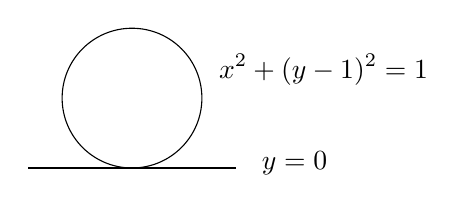
\begin{tikzpicture}[x=0.75pt,y=0.75pt,yscale=-1,xscale=1]
			%uncomment if require: \path (0,300); %set diagram left start at 0, and has height of 300
			
			%Straight Lines [id:da9022525264933119] 
			\draw    (44,106) -- (144,106) ;
			%Shape: Circle [id:dp5620106547865036] 
			\draw   (60.33,72.33) .. controls (60.33,53.74) and (75.41,38.67) .. (94,38.67) .. controls (112.59,38.67) and (127.67,53.74) .. (127.67,72.33) .. controls (127.67,90.93) and (112.59,106) .. (94,106) .. controls (75.41,106) and (60.33,90.93) .. (60.33,72.33) -- cycle ;
			
			% Text Node
			\draw (155.33,97) node [anchor=north west][inner sep=0.75pt]   [align=left] {$\displaystyle y=0$};
			% Text Node
			\draw (134.67,50) node [anchor=north west][inner sep=0.75pt]   [align=left] {$\displaystyle x^{2} +( y-1)^{2} =1$};
		\end{tikzpicture}
	\end{center}
	
	直观上, 直线与圆相切, 两者在相切处有一条公共的 ``无穷小线段''. 更一般地, 任意两条相切的曲线都有一条公共的形如 $D$ 的无穷小线段, 这便是两条曲线共同的切向量.
\end{example}

\subsection{Kock--Lawvere 公理}

\begin{axiom}
	{(Kock--Lawvere 公理)}
	对任意映射 $f \colon D \to R$, 存在唯一的 $a,b\in R$,
	使得
	$$
	f(d) = a + d\cdot b,\quad\forall d\in D.
	$$
\end{axiom}

Kock--Lawvere 公理反映了如下的直观: $R$ 上的一个函数在一个很小的邻域上近乎是一次函数.
由此, 我们立刻得到如下的推论.

\begin{propdef}
	{(导函数)}
	对任意函数 $f\colon R\to R$, 存在唯一的函数 $f' \colon R \to R$ 满足
	$$
	f(x+d) = f(x) + d \cdot f'(x),\quad \forall x\in R\,\forall d\in D.
	$$
	称 $f'$ 为 $f$ 的\emph{导函数}. 归纳地定义 $k$ 阶导数 $f^{(k)}(x)$.
\end{propdef}

任何函数都是任意次可导的.

\subsection{综合微分几何的模型}

\todo{光滑环}